\section*{Appendix A: Compactified Dimensional Architecture in Recursive Cosmology}

\subsection*{A.1 Dimensional Framework}

We posit that the recursive cosmology framework arises from an 11-dimensional M-theoretic bulk, with one emergent informational dimension, yielding a 12-dimensional extended configuration space~\cite{witten1995string, becker2007string}:

\begin{itemize}
  \item \textbf{4 macroscopic spacetime dimensions}: $(t, x, y, z)$.
  \item \textbf{6 compactified Calabi-Yau dimensions}: encoded via topological moduli, e.g., complex structure and Kähler parameters~\cite{candelas1985vacuum}.
  \item \textbf{1 informational dimension} $\mathcal{I}$: representing entanglement flux or coherence memory.
  \item \textbf{1 holographic boundary dimension}: supporting inter-cycle projection and encoding~\cite{ryu2006holographic}.
\end{itemize}

\begin{figure}[H]
\centering
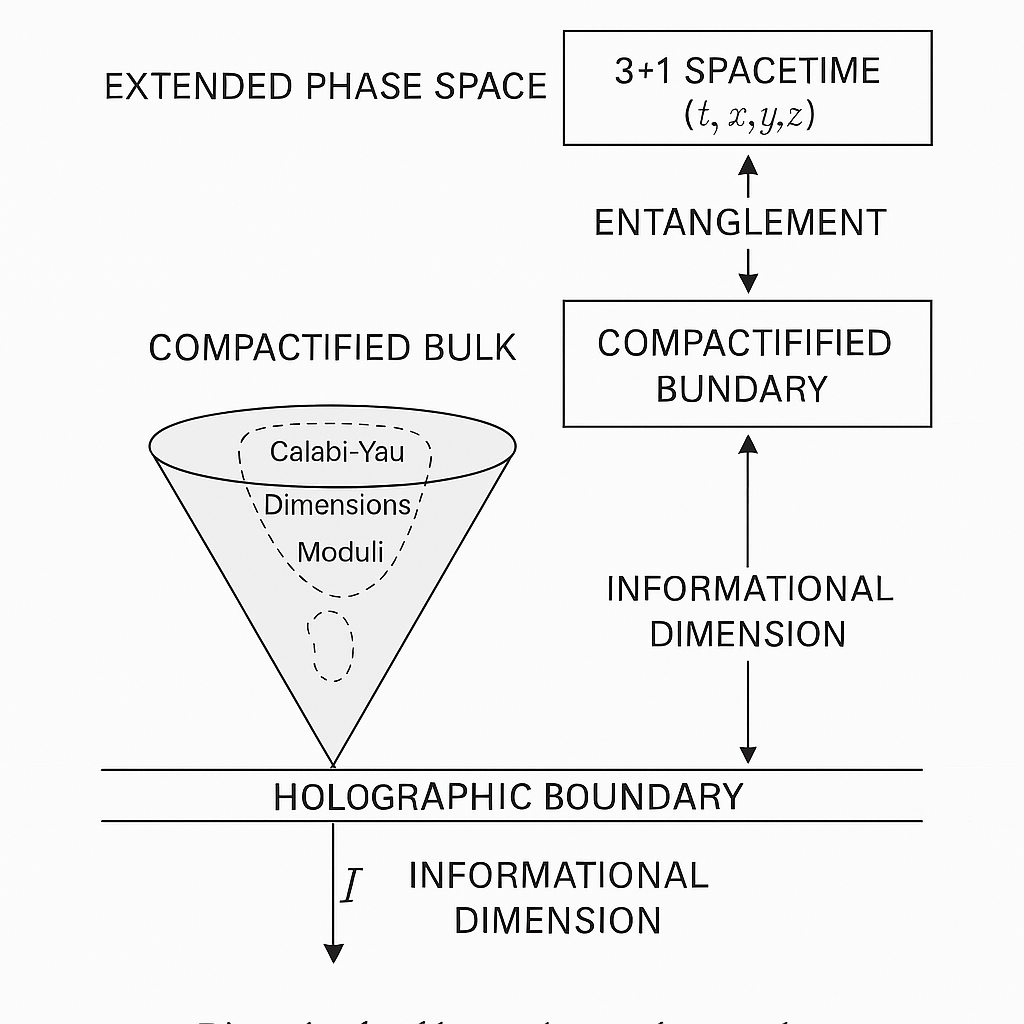
\includegraphics[width=0.75\textwidth]{figures/12D_structure_diagram.png}
\caption{Schematic of the proposed 12-dimensional recursive configuration space structure.}
\label{fig:12D_structure}
\end{figure}

\subsection*{A.2 Boundary Geometry}

Each cosmological cycle terminates on a boundary $\Sigma_n$, defined by minimal-area surfaces derived from quantum extremal surface (QES) conditions~\cite{engelhardt2015coarse}:

\[
\Sigma_n = \arg\min_{\partial \mathcal{M}} \left( \frac{\mathrm{Area}[\partial \mathcal{M}]}{4G_N} + S_{\text{bulk}} \right)
\]

where $S_{\text{bulk}}$ is the von Neumann entropy of the entanglement wedge. Information from $\Sigma_{n-1}$ is holographically projected into $\Sigma_n$, preserving partial memory between cycles~\cite{almheiri2019entropy}.

\subsection*{A.3 String-Theoretic Justification}

In the M-theoretic embedding, inter-cycle information transfer occurs via Planck-scale excitations along wrapped branes across compact dimensions. The Einstein-Rosen bridge (ERB) throat corresponds to a minimal energy wormhole solution supported by tensionless M2-branes~\cite{maldacena2013cool}:

\[
S_{\text{ERB}} \sim \frac{A_{\text{min}}}{4G_N} + i \lambda_E I(\phi, \phi')
\]

These excitations source the interference phase in the recursion kernel.

\subsection*{A.4 Observational Consequences of Compact Geometry}

The Calabi-Yau moduli induce spectral oscillations in the gravitational wave background through modulated bounce dynamics. Frequencies $f_j$ are harmonics of the compactification scale $L_c$~\cite{dienes1997string}:

\[
f_j \sim \frac{j}{L_c}, \quad j \in \mathbb{Z}^+
\]

These modulations are expected to appear as resonant dips or harmonics in $\Omega_{\text{GW}}(f)$, potentially observable by future gravitational wave detectors.

\subsection*{A.5 Summary}

This embedding allows the recursive decoherence kernel and ERB-mediated memory propagation to emerge naturally from the compactified geometry. The 12-dimensional structure is not metaphysical—it arises from established string-theoretic geometry, entanglement propagation, and holographic boundary dynamics. The informational dimension is a mathematical representation of recursive coherence flow, grounded in entanglement entropy and bulk/boundary duality. No additional assumptions beyond known M-theoretic constructions are invoked.
